\chapter{Обзор предметной области}

Чтобы достичь намеченных целей, необходимо понять, что из себя представляет экран мобильного приложения, а также из каких элементов может состоять его интерфейс.

\section{Основные понятия}
В iOS существует различие между координатами, указываемыми в коде, и пикселями устройства \cite{pixel} -- наименьшими дискретными элементами двумерного цифрового изображения. Для большинства задач фактический размер точек \cite{point} не имеет значения, их цель -- обеспечить согласованный масштаб, который может использоваться в коде для указания размера и положения представлений и отображаемого содержимого. Например, если пиксели в два раза меньше изначальной высоты или ширины, можно использовать квадрат 2×2 пикселя для каждой точки (это называется масштаб @2x). Таким образом, измерение в точках позволяет корректно масштабировать изображение на экранах с высоким разрешением. \cite{hig}

\begin{figure}[h!]
	\centering{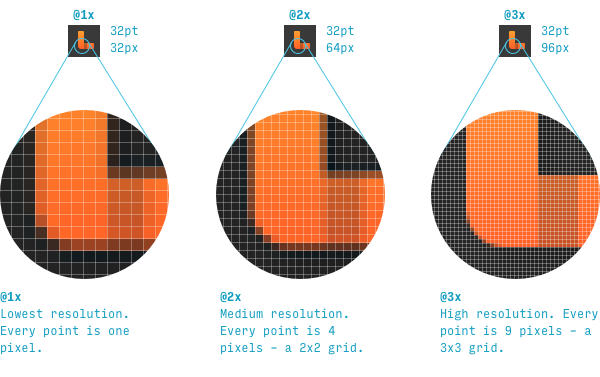
\includegraphics[scale=0.75]{img/point.png}}
	\caption{Точки и пиксели}
	\label{fig:points}
\end{figure}

Устройства, работающие на операционной системе iOS, имеют различное разрешение экрана и соотношение сторон. Так, например, iPhone X имеет разрешение 1125 x 2436 пикселей и коэффициент масштабирования в точки, равный 3.0 (то есть 375 x 812 точек), а iPhone 6  -- 750 x 1334 пикселей и коэффициент 2.0 соответственно (то есть 375 x 667) \cite{displays}. А также каждое устройство имеет горизонтальную и вертикальную ориентацию. Данные характеристики стоит учитывать в разработке, дабы создавать приложения, интерфейс которых адаптируется к устройствам разного размера, а также любой их ориентации. 

\section{UIKit}

UIKit \cite{uikit} -- библиотека, предоставляющая архитектуру окон и представлений для реализации пользовательского интерфейса, включая компоненты, которые можно использовать для построения базовой инфраструктуры приложения. Альтернативой выступает фреймворк SwiftUI \cite{swiftui}, предоставляющий не меньше возможностей, однако, будучи представленным в 2016 году, библиотека не смогла стать столь популярной в разработке. Поэтому целесообразным будет рассмотреть методы верстки UI-элементов, предоставляемых UIKit.


Рассмотрим базовые UI-элементы, предоставляемые фреймворком UIKit.

UIView (или представление) \cite{uiview} -- это фундаментальный блок пользовательского интерфейса приложения, а UIView-класс определяет поведение, общее для всех представлений. Объекты этого класса отображают содержимое в пределах своих границ и обрабатывают любые взаимодействия с этим содержимым. Для отображения надписей, изображений, кнопок и других элементов интерфейса, обычно встречающихся в приложениях, используют не определяемые самостоятельно подклассы view, а предоставляемые платформой UIKit. 

UIViewController (или контроллер) \cite{controller} -- объект, который управляет иерархией представлений приложения. Основные обязанности контроллера включают следующее:

\begin{itemize}
	\item обновление содержимого представлений;
	\item реагирование на взаимодействие пользователя с представлениями;
	\item изменение размеров представлений и управление макетом общего интерфейса;
	\item координация с другими объектами, включая другие контроллеры представления.
\end{itemize}

Итак, экран в мобильной разработке представляет UIViewController, являющийся контейнером для других UIView. Труд команды разработки интерфейса мобильного приложения сводится к задаче корректного отображения элементов на экране -- расположения UIView на UIViewController. Чтобы работа была эффективной, целесообразно каждому члену команды дать индивидуальную подзадачу -- таким образом используемая технология верстки должна предполагать возможность работы нескольких участников над одним проектом и минимизировать количество ошибок, возникающих при изменении параметров UI-элементов. 

На основе рассмотренных теоретических сведений можно выделить критерии, по которым необходимо провести анализ эффективности использования методов верстки:

\begin{itemize}
	\item возможность создания интерфейса, масштабируемого для устройств разного размера и двух ориентаций экрана, и относительная сложность его создания;
	\item сложность командной разработки интерфейса; (сложность?)
	\item сложность внесения изменений в интерфейс;
	\item возможность обработки всех параметров UI-элемента;
	\item порог входа в технологию метода и ее наглядность; ???
	\item скорость работы метода.
\end{itemize}

Рассматривать разные элементы?

\chapter{Методы верстки}

Под понятием разметки подразумевается расчет необходимых координат и размеров UI-элементов.
Существует два основных подхода к созданию пользовательского интерфейса: можно программно компоновать элементы, задавая координаты и размеры каждого в коде, или же использовать автоматическую компоновку.

\section{Ручная верстка}

\subsection{Frame}

Frame \cite{frame} -- свойство view, описывающее прямоугольник, определяющий местоположение и размер представления в системе координат его родительского view \cite{superview}.

\begin{figure}[h!]
	\centering{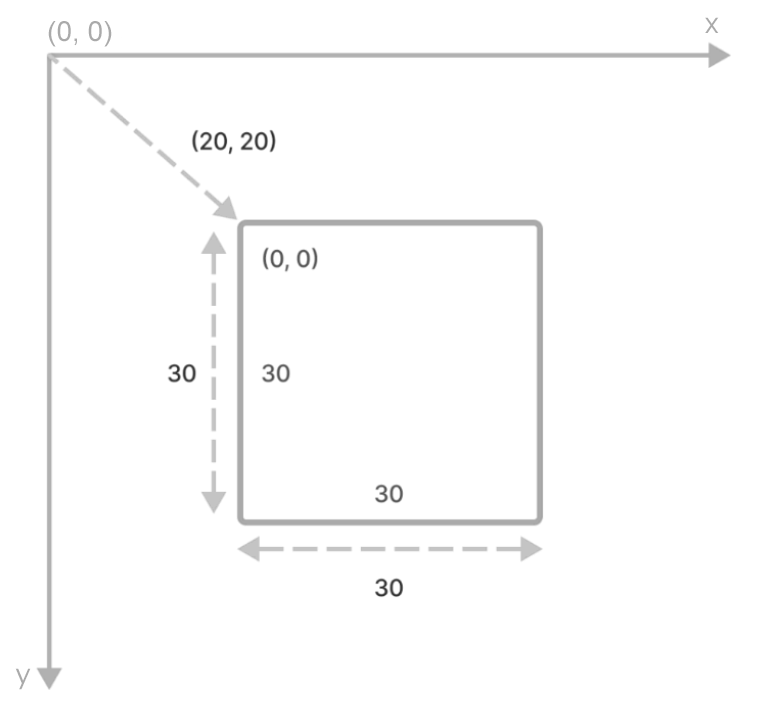
\includegraphics[scale=0.65]{img/frame.png}}
	\caption{Frame}
	\label{fig:frame}
\end{figure}

View, представленную на рисунке 2.1, можно описать кодом, представленным в листинге 2.1. 

%\hspace{0.6cm}В Листинге представлен задание свойства frame для UIView.
\begin{lstlisting}[caption=Задание свойства frame для UIView]
	var view = UIView()
	view.frame = CGRect(x: 20, y: 20, width: 30, height: 30)
\end{lstlisting}

Ручная верстка предполагает задание кодом координат и размеров каждого элемента экрана. Указание координат идет относительно левого верхнего угла экрана -- именно там располагается точка (0, 0). При желании запустить будущее приложение на двух устройствах, размеры экрана которых различны, результат также будет разниться. То же будет происходить и при попытке сравнения экранов горизонтальной и вертикальной ориентации. Таким образом, возникает необходимость вручную обрабатывать каждый из возможных размеров дисплея в двух вариациях ориентации. На данный момент существует 10 различных размеров экрана iPhone и 7 -- iPad. Нетрудно представить, во сколько раз увеличиватся количество строк кода и повышается трудоемкость задачи при обработке каждого случая. 

Однако данный подход позволяет разбить задачу создания интерфейса на несколько подзадач, поскольку в пределах одной superview разработчик взаимодействует лишь с этим родительским представлением и конкретной view. Внесение изменений в написанный раннее код также не составит большого труда, так как параметры, задаваемые в свойстве frame, независимы друг от друга и их значения являются константами.

При использовании данного метода разметки разработчик получает возможность создания любого кастомного элемента, поскольку имеет доступ к обработке каждого визуального параметра UI-элемента. Так, например, можно задавать радиус угла view, цвет и прозрачность элемента, что представлено в листинге 2.2.

\begin{lstlisting}[caption=Задание параметров view]
	var view = UIView()
	view.frame = CGRect(x: 20, y: 20, width: 30, height: 30)
	view.layer.cornerRadius = 2.0
	view.backgroundColor = UIColor.red.withAlphaComponent(0.5)
\end{lstlisting}

Для того, чтобы оценить время работы метода, необходимо упомянуть, что любые модификации UI-элементов производятся на главном потоке многопоточного приложения -- main thread \cite{mainthread}. Поскольку параметрами свойства frame выступают константа, а, соответственно, никакие вычисления не производятся, скорость работы метода будет соответствовать скорости размещения элементов на экране. 


\section{Автоматическая верстка}

Существует альтернативный способ расчета необходимых координат и размеров. 

Автоматическая компоновка (или Auto Layout) \cite{autolayout} динамически вычисляет размер и положение всех видов в иерархии на основе ограничений, наложенных на эти view. Например, существует возможность ограничить кнопку так, чтобы она была центрирована по горизонтали в соответствии с видом изображения и ее верхний край всегда оставался на 8 точек ниже нижнего края изображения. 

Правила (или constraints), задаваемые Auto Layout, представляют собой обычное линейное уравнение вида \begin{equation}
	y = a \cdot x + b,
\end{equation}
где y – необходимая координата или размер; a – произвольный множитель; x – параметр, от которого зависит итоговый результат; b – константа. Для того чтобы корректно посчитать координаты и размер элемента, необходимо минимум 3 правила, которые сложатся в систему равнений, результатом решения которой будут координаты и размер элемента.

Существует два основных способа задать ограничения для автоматической компоновки: программный, когда каждое ограничение представлено строкой кода, и автоматический, когда ограничения заданы с помощью инструмента работы с пользовательским интерфейсом Storyboard \cite{storyboard}.

\subsection{Auto Layout программно}


\subsection{Storyboard}

